%\documentclass[titlepage,a4paper,12pt]{book}
%\usepackage[utf8]{inputenc}
%\usepackage[catalan]{babel}
%\usepackage{graphicx}
%\usepackage{marvosym}
%\usepackage{listings}
%\usepackage{textcomp}
%\usepackage[]{color}
%\begin{document}
%\tableofcontents

\chapter{Algoritmes genètics}
\label{cha:AG}

En aquest capítol es farà una repàs de que es coneix com algorismes evolutius
\cite{H75}. S'explicarà una de les dos filosofies existents,
algorismes genètics darwinistes (GA) i es farà una introducció a Genetic
Expression programming (GEP), on per explicar aquest segon tipus d'algorismes
s'introduiran els algorismes de programació genètica (GP), que és l'origen del
que va partir GEP.

\section{Introducció}
Els algorismes genètics són eines evolutives, que es poden
classificar dins del camps de la intel·ligència artificial i que es solen usar
en problemes d'optimització. La filosofia d'aquesta família d'algorismes és
basar-se en els mecanismes de selecció natural que Darwin ja va presentar en el
llibre \emph{The Origin of Species}, és a dir, els individus que millor
s'adapten a l'entorn són aquells que sobreviuen amb major facilitat.
Conseqüentment també produeixen més descendència, la qual cosa provoca que, de
mica en mica, els trets diferencials que caracteritzen als bons individus es van
propagant per la població i a través dels seus descendents.

En els algorismes evolutius, les solucions al problema són codificades com a
individus d'una població, tal i com es veurà més endavant.  Posteriorment,
simulant les diferents fases per la que passa la reproducció natural, i aplicant
tècniques que provoquen un cert grau de pressió selectiva (supervivència dels
més forts), aquestes van evolucionant cap a solucions al problema més bones.
Els primers fonaments dels algorismes genètics van ser proposats per Holland \cite{H75} al 1975.
Aquests algorismes aconsegueixen evolucionar els individus de tal manera que el
grau d'adaptació a l'entorn (avaluació o \emph{fitness}) va augmentant de
generació en generació.

\section{Algorismes genètics darwinistes}

Els algorismes genètics Darwinistes segueixen l'esquema de funcionament clàssic
dels algorismes genètics. En aquests, s'intenta imitar els processos de la
evolució natural sense cap altra modificació conceptual.  Normalment, quan es
parla del terme algorisme genètic es refereix a aquest model de
funcionament. En l'actualitat els algorismes genètics han estat molt utilitzats
en gairebé tots els àmbits de la ciència com a eina per optimitzar o buscar
bones solucions comparables a les actualment disponibles.  L'àmbit de la
bioinformàtica és una de les àrees d'aplicacions reals on s'han utilitzat algorismes genètics amb
més èxit \cite{PSBE01,D96,wgl:2000,WWBG95}.

\subsection{Principis bàsics}

Els algorismes genètics es recolzen en tres pilars bàsics: el primer d'ells és
la selecció d'individus de la població, el segon el creuament d'individus i el
tercer la funció d'avaluació. La selecció és important perquè és el mètode per
escollir els individus que generaran descendència, seria bo que normalment
aquests individus fossin els millors adaptats a l'entorn. És a dir, aquells amb
un \emph{fitness} més alt.  Això, junt amb el creuament de les solucions
seleccionades, progressivament fa evolucionar la població de solucions. La
funció d'avaluació és el mecanisme amb el qual es computa el grau d'adaptació de
cada individu a l'entorn.

Del paràgraf anterior es pot deduir que els algorismes genètics són algorismes no deterministes.
Això és el resultat dels mecanismes estocàstics emprats. I això pot comportar
que no sempre s'assegura l'obtenció del màxim global de la funció que es vol
optimitzar, la qual cosa és certa, però el que sí que s'ha demostrat
empíricament és que normalment sempre s'arriben a solucions bones amb un temps
molt menor que hagués trigat un algorisme de cerca sistemàtic \cite{BBM93}. 

\subsubsection{Representació dels individus}

Continuant amb les analogies biològiques, la representació de les solucions es
fa emprant cromosomes. Aquests estan formats per la concatenació de gens. Cada
gen representa el valor d'un paràmetre (o variable de decisió) d'una possible
solució.  Per exemple, si estem definint les proporcions òptimes per a una
caixa, un cromosoma podria venir definit per les següents variables:
(altura ,amplada, profunditat). Cada solució hauria d'estar perfectament definida
en el seu cromosoma.

Al cromosoma també se'l coneix com \emph{genotip}, ja que representa un conjunt de
qualitats o atributs de la solució que no s'expressen en la realitat (en aquest
cas la realitat s'entén com la simulació necessària per avaluar un cromosoma).

Podria ser que l'hora de simular el cromosoma, s'adoptaren una serie de
qualitats no definides al cromosoma de forma aleatòria, o indeterministes.
Aquestes qualitats que surten a la llum al ``avaluar'' un element, formen part
del \emph{fenotip}.  Per d'exemple, es pot imaginar un cromosoma o genotip on
els seus gens són els Cadenes d'àtoms que unim a un cert esquelet d'una
molècula\cite{GEB79}. El fenotip serà l'estructura tridimensional que aquesta
molècula adoptarà a l'espai, que no necessàriament ha d'estar codificada al
cromosoma.

\subsubsection{Esquema bàsic}

Com s'ha comentat anteriorment, un algorisme genètic imita el cicle de la
evolució natural proposat per Darwin. Aquest cicle bàsicament es pot resumir en
cinc fases: inicialització, avaluació, selecció, creuament i mutació. Cadascuna
de les quals es descomposa en altres subfases que seran explicades en la secció
\ref{subsec:operadors}. La figura \ref{fig:ga} es mostra el diagrama
d'activitats que segueix un GA.

\begin{figure} \centering 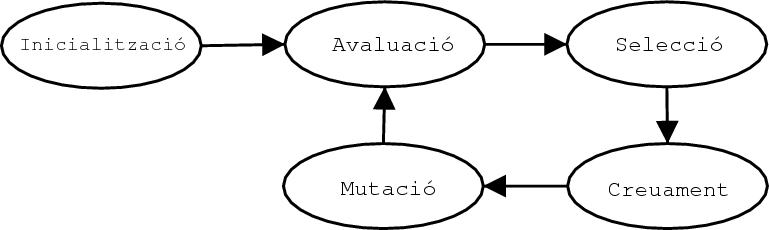
\includegraphics[width=4in]{intro/ga}
\caption{\label{fig:ga}Diagrama d'activitats d'un algorisme genètic}
\end{figure}

A grans trets, la fase d'inicialització, crea la població inicial que començarà
el procés evolutiu. Sempre cal un conjunt suficientment gran i divers per
assegurar l'èxit del procés evolutiu \cite{G02}.

Pel que fa a l'avaluació, cal dir que és un dels aspectes més importants d'un
GA, en l'apartat \ref{subsec:avaluacio} s'entrarà amb molt més detall amb aquest
afer, però cal comentar abans que la funció d'avaluació és en si mateix el
problema que es vol resoldre o optimitzar.

La selecció és el mecanisme que tria els individus que seran candidats a ser
escollits, més endavant s'entrarà en molt més detall en els mecanismes
involucrats en la selecció desenvolupada, i també es citaran altes tècniques de
selecció.

El creuament és el procés pel qual es combinen dos cromosomes que s'han
seleccionat per tenir descendència. Hi han moltes formes de fer-ho, però una de
les més habituals és un creuament discret amb un o dos punts de tall.  Aquesta
és la tècnica que hem usat en dos dels nostres projectes \texttt{Pholus} i
\texttt{Chiron}  %% refs

Finalment, vé la mutació, que és l'encarregada d'introduir o canvis aleatoris en
els individus amb una probabilitat més aviat baixa. Aquesta activitat és
realitza per estar segurs de que tot l'espai de cerca pugui ser explorat.
Modificant la probabilitat d'aparició de mutacions donem més o menys
variabilitat genètica al algorisme, afavorint o desfavorint la convergència de
la població.

En acabar la mutació el cicle es tanca, i va iterant fins que la condició
d'aturada s'assoleix. Normalment la condició d'aturada és generar un nombre
prefixat de generacions, però alguns cops també s'utilitzen criteris, com per
exemple la convergència de la població.

\subsubsection{La funció d'avaluació\label{subsec:avaluacio}} La funció
d'avaluació és vital per un algorisme genètic. Aquesta tracta de simular
l'entorn en el qual estan immerses les solucions, i ens retorna el
\emph{fitness} o el grau d'adaptació dels individus a l'entorn. Cal fer notar
que la funció d'avaluació codifica el problema que es vol que el GA resolgui.

En alguns problemes la funció d'avaluació és tan complexa que s'ha de
simplificar per aproximacions més ràpides. Fins i tot en alguns casos s'ha
observat que el fet de substituir la funció d'avaluació per una menys complexa
dóna la oportunitat d'avaluar més individus per unitat de temps, i amb aquest
increment dels individus avaluats, al final s'assoleix una solució real més
acurada que la que es va trobar utilitzant la funció d'avaluació inicial
\cite{G89}. 

\subsubsection{Reproducció} En la reproducció estan implicats dos dels tres
pilars fonamentals dels GA, la selecció i el creuament. La creació de nova
descendència és un factor crític, en la mesura que de generació en generació,
els nous individus creats van superant als seus ascendents.

A partir d'ara entra en joc el concepte de pressió selectiva. És a dir, la
pressió que d'alguna manera s'exerceix sobre la població per a que vagi
augmentant el seu grau d'adaptació a l'entorn. Sovint s'ha de vigilar amb la
pressió selectiva, per que si és massa elevada, l'algorisme no té altra
escapatòria més que arribar a solucions bones a curt termini però que no
assoleixen els màxims globals. Aquestes solucions queden estancades en màxims
locals. D'altra banda si la pressió selectiva és molt baixa, el temps de
convergència és molt llarg.  Com sempre, s'ha d'arribar a un nivell de
compromís, entre el temps de convergència i el risc de caure en màxims locals.

Cal fer notar que de vegades podria ser que alguns individus siguin seleccionats
repetits cops en una mateixa generació. Això no té per que ser dolent, ja que
normalment aquests tipus d'individus tindran un \emph{fitness} molt alt.

Quan els individus que van a ser creuats ja han estat seleccionats, sols queda
pendent emparellar en grups de dos els individus per tal de generar nova
descendència. 

Un concepte que també s'ha d'introduir és el concepte d'\texttt{elitisme}, que
implica guardar els $k$ millors individus de la població de generació en
generació, així s'assegura que els millors individus de la població no es perden
mai.  Aquest és un element que afegeix pressió evolutiva, mantenint un ``llistó''
del que no es baixa mai generació a generació, i accelerant la convergència.

\subsubsection{Convergència} 

Normalment els individus d'un GA van convergint cap als màxims de la solució de
generació en generació. Es diu que un GA ha convergit quan el 95\% de la
població té el mateix valor \cite{D75}, i una població ha convergit quan tots
els seus gens han convergit.

En alguns casos la condició d'aturada del cicle d'activitats d'un GA ve imposat
per condicions de convergència.  Quan els individus han assolit un cert nivell de
convergència (el 95\% dels individus d'una generació són iguals), en general
implica que el GA no evolucionarà més les solucions, per tant té sentit aturar
la cerca.

Quan apliquem operadors (veure secció \ref{subsec:operadors}) molt restrictius,
que donen molta pressió evolutiva, ens podem trobar en casos de
\emph{convergència prematura}, és a dir, en poques generacions, tots els
individus s'assemblen massa entre ells i els creuaments són poc efectius.  En
aquests casos, l'algorisme s'estanca en un màxim o mínim local, però rarament
global.

\subsection{Operadors\label{subsec:operadors}} 

S'entenen com els operadors d'un GA com les diferents tècniques de realitzar les
5 fases bàsiques d'un GA. En el treball final de carrera titulat com
\emph{Química combinatòria virtual: disseny de pèptids que travessen la barrera
hematoencefàlica} \cite{B01},  hi ha un ampli recull d'operadors, on s'analitzen
els punts forts i febles de cadascun.  A continuació es descriuen els operadors
emprats en el GA desenvolupat en aquest projecte en cadascuna de les fases.

\subsubsection{Inicialització} 
\label{ssub:IInicialitzacio}

Per fer les inicialitzacions es poden descriure molts mètodes, des de models
totalment aleatoris, fins a la incorporació de certes heurístiques o coneixement
sobre el problema. En aquest projecte s'ha optat per una inicialització
aleatòria, sempre i quan els cromosomes compleixin amb els requeriments del
problema.  Com s'explica en cadascun dels apartats, cada gen pot prendre un
nombre finit de valors, o com a màxim, un rang (en el cas de ser representat per
un real).

\subsubsection{Selecció}
\label{subs:Iseleccio}
La selecció és la manera en que s'escolliran els individus de la població més
ben adaptats, per a permetre que aquests siguin els ``pares'' dels individus de
la següent generació.

La selecció, en els algorismes evolutius és típicament probabilística, donant
més probabilitats de ser ``pares'' als cromosomes de més qualitat que als de
menys.  De totes maneres, els individus de poca qualitat també tenen alguna
possibilitat d'encreuar-se i així passar el seu ``codi genètic'' a generacions
futures.

Tècniques de selecció n'hi ha moltes, i aquí n'explicarem només algunes, les
que hem provat per als nostres projectes, o bé alguna d'especialment curiosa.

Els \emph{fitness proportional selection}, també anomenat selecció per ruleta
basen el seu funcionament en què per a cada selecció, la probabilitat que un
individu $f_i$ sigui seleccionat per a reproduir-se depèn únicament del seu
\emph{fitness} absolut comparat amb els fitness dels altres individus de la
població (Figura \ref{fig:rwsgraph}).

Aquest mecanisme de selecció va ser introduït a \cite{H75} i ha estat molt
estudiat en endavant.  Donada la seva simplicitat, s'han trobat diversos
problemes:

\begin{itemize}
	\item Els individus que són molt més bons que la resta, tendeixen a
	``conquerir'' la població sencera molt ràpidament. Provoca convergència
	prematura.
	\item Si els fitness dels individus són molt similars, la pressió selectiva
	es veu molt mermada, fent que a la hora d'escollir, es tingui gairebé les
	mateixes probabilitats d'escollir un individus que un altre, fent que la
	selecció segueixi una distribució uniforme aleatòria.
\end{itemize}


\begin{figure} \centering 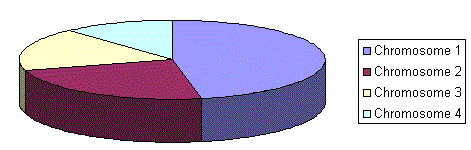
\includegraphics[width=4in]{intro/rwsgraph.png}
\caption{\label{fig:rwsgraph}Ruleta FPS}
\end{figure}

La selecció \emph{basada en ranking}, és un altre mètode que intenta
solucionar els problemes de FPS \cite{B87a}.  Aquest mètode manté la pressió
selectiva ordenant la població en funció del seu fitness, i assignant les
probabilitats de selecció en funció de la ordenació en comptes de fer-ho en
funció del propi fitness. D'aquesta manera, s'estableix una relació de qui és
millor que qui, però no hi ha els problemes que teníem en FPS.  El problema que
té aquest mètode és que no fa cap distinció entre les relacions de fitness
excepte per la relació de ser millor que un altre.  Per exemple, tres elements
amb fitness 1,2,3 s'ordenaran igual, i amb les mateixes probabilitats de ser
seleccionats que elements amb fitness 1,100 i 1000 .  La manera que es té de
mitigar (que no solucionar) aquest problema és assignar proporcions escalades en
relació entre la posició en el ranking i la probabilitat de ser seleccionat,
pot ser una relació lineal, exponencial o bé logarítmica. 

En la figura \ref{fig:rank1} es mostra  un cas on hi ha un cromosoma que tindria
el 90\% de probabilitats de ser escollit. El que es fa és ordenar de pitjor a
millor, i al pitjor donar-li un ``calaix'', al següent dos, al següent tres, i
finalment, al millor quatre. 

\begin{figure} \centering 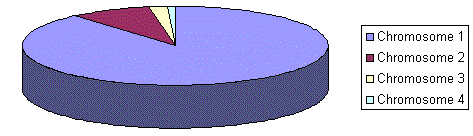
\includegraphics[width=4in]{intro/rank1.png}
\caption{\label{fig:rank1}selecció ranking}
\end{figure}

En casos reals, s'utilitzen sistemes una mica més sofisticats, com per exemple
la \emph{selecció per torneig}.  En una selecció per torneig s'ha de definir
un paràmetre $N$ que descriu la mida del torneig.

En la selecció per torneig, per decidir quin individu passarà a la següent
generació, es realitzen ``enfrontaments'' de $N$ individus, comparant el seu
fitness.  El que guanya de tots ells serà qui passarà a la fase de creuament.

Una de les avantatges que té aquest mètode és que no fa falta tenir
comptabilitzats tots els fitness de la població sencera, ja que només s'han
d'avaluar per grups de $N$.  Això el fa molt còmode d'usar en sistemes
paral·lelitzats, o bé en problemes on es molt costós fer una ordenació dels
fitness a nivell global, com per exemple, quan avaluem tirades en un joc
estratègic.

Hi ha variants de tornejos on, es defineix un altre paràmetre, que és la
probabilitat que el que té millor fitness surti realment guanyador.  En els
tornejos normals (deterministes), aquest paràmetre $p=1$, però si el disminuïm
tal que $p<1$, hi haurà un numero de casos $1-p$ on no guanyarà el millor.
Aquesta tècnica redueix la pressió evolutiva permetent que individus pitjors,
passin el seu codi genètic a següents generacions, augmentant la diversitat.

L'algorisme esquematitzat (tant per p=1 com per p<1) és el següent:

\begin{itemize}
	\item S'escullen $N$ individus de la població aleatòriament.
	\item S'agafa el millor individu amb probabilitat $p$.
	\item S'agafa el segon millor individu amb probabilitat $p \times (1-p)$
	\item S'agafa el tercer millor individu amb probabilitat $p \times (1-p)^2$
	\item \ldots
\end{itemize}


%En aquest projecte s'ha utilitzat una selecció \emph{stochastic
%universal samplig} \cite{B87a} amb \emph{rank selection} \cite{B87b} i una
%tècnica d'especiació coneguda com \emph{sharing} \cite{33}.

\subsubsection{Creuament}

Un cop s'han seleccionat els individus de la nova població, aquests podran tenir
descendència. Per a cadascun d'ells es genera un nombre aleatori entre 0 i 1, i
si no supera una determinada probabilitat de creuament, normalment bastant alta,
és copiat directament a la següent fase que és la mutació.

Els individus escollits per creuar-se són agrupats en parelles aleatòries, i
s'aplica un creuament clàssic discret unipunt.  Es genera un punt de tall del
cromosoma de forma aleatòria, i es construeixen dos descendents. El primer
descendent contindrà la primera part del material genètic del primer progenitor
fins el punt de tall, i la segona part del segon progenitor, que va des del punt
de tall fins el final del cromosoma. El segon descendent serà a l'inrevés, la
primera part serà directament la primera part del segon progenitor, i la segona
part la segona del primer progenitor.

En els dos problemes de GA hem utilitzat el creuament unipunt, però també hi
ha variants d'aquest creuament utilitzant dos o més punts.  Com es veurà en les
seccions de cadascun dels problemes, s'han fet proves amb aquests creuaments,
però no ens han donat resultats millors, i hem seguit amb els creuaments
unipunt.

Aquests creuaments, es poden aplicar amb seguretat quan considerem que la
relació d'un gen $i$ amb el gen $i+1$ no és forta (no hi ha epistàcia).  Si
trencant un cromosoma per la posició $i$, destruïm algun \emph{building block},
probablement, es perdrà un factor que feia que l'individu fós bo, i al
creuar-lo, no obtindrem gaire bons resultats.

\subsubsection{Mutació}

Finalment, abans de tancar el cicle, es realitza la mutació. Aquesta activitat
aplica mutacions de forma aleatòria, però amb una baixa probabilitat, als gens
dels individus de la nova generació que està a punt de crear-se. En el cas de
disposar d'elitisme, aquests individus no són exposats a les mutacions.

L'operador de mutació emprat és clàssic uniforme. Això implica que els gens
seleccionats per a ser mutats, se'ls canvia el seu valor de forma aleatòria
però, el nou valor pertany al domini de la variable de decisió que codifica
aquell gen.

\subsubsection{Reemplaçament}

El model de reemplaçament seleccionat és el conegut com elitisme, que com ja
s'ha explicat abans, crear tota una nova població d'individus de generació en
generació. Malgrat això els $k$ millors individus van guardant-se per tal
d'assegurar que no es perden al llarg del procés evolutiu.  En tots els
projectes que es presenten en aquest treball, s'ha mantingut la mida de la
població, però també es possible fer que aquesta mida de la població varii al
llarg de les generacions.

%\subsection{Teoremes} En general no n'hi ha cap teoria universalment acceptada
%del perquè funcionen bé els GA, ni del perquè de la seua robustesa. Però n'hi
%han dues hipòtesis que són interessants conèixer per que ens poden ajudar a
%implementar bones aplicacions dels GA, i cada cop més estan adoptant-se pels
%teòrics com els vertader mecanismes que fan evolucionar els GA. El primer
%d'ells és el teorema de la disposició, i el segon la hipòtesi dels blocs de
%construcció, o \emph{building blocks}.

%\subsubsection{Teorema de la disposició} Més conegut per \emph{schema theorem},
%va ser proposat per Holland \cite{H75}. Un \emph{schemata} és un patró de
%valors dels gens en binari. On aquest patró està format \{1, 0, \( \star  \)\}
%sent \( \star  \) el caràcter comodí. De tal forma que cromosomes com
%{}``0000'', {}``0010'', {}``0001'' i {}``0011'' corresponen al mateix patró
%{}``00\( \star \star  \)''.

%Aquest teorema diu que els individus bons, ho són per que tenen un bon patró.
%Llavors hem de donar-los a aquests individus més possibilitats de reproducció
%en funció del seu \emph{fitness}.  Per tant al passar aquests patrons a la
%descendència i al aplicar-los aquest mateixa filosofia, anem augmentant les
%possibilitats de generar millors patrons a mesura que passa el temps.

%Segons Holland si distribuïm aquestes probabilitats en funció de la proporció
%del \emph{fitness} d'un individu a seleccionar front al de la resta, un bon
%patrons estarà tenint un nombre de possibilitats que va creixent
%exponencialment. També va dir que el nombre de patrons que estant sent
%processats en una generació, és n\( ^{3} \), on n és el tamany de la població.
%Això és conegut com paral·lelisme implícit.

%\subsubsection{Hipòtesi sobre els blocs de construcció \label{subsec:bb}}
%Goldberg, en canvi, formula la \emph{Building Block Hypotesis} \cite{G89}.  Que
%diu que la potència dels GA's recau sobre l'habilitat de crear bons blocs de
%construcció. Aquests són curts patrons amb una longitud fixa, que funcionen
%molt bé per separat; independentment de la resta del cromosoma. I que si se li
%és incorporat un bon bloc de construcció a un cert individu, el seu
%\emph{fitness} augmenta. 

%Per afavorir la aparició de blocs de construcció, la codificació del cromosoma
%hauria de tenir propers els gens relacionats, i al mateix temps, que la
%interacció entre els gens siga mínima.

%La no interacció entre gens vol dir que l'aportació d'un gen al còmput del
%\emph{fitness} no es vegi afectat per els valors que poden prendre altres gens.
%Més tard Goldberg va publicar els estudis teòrics sobre gens que sí que
%interaccionen entre ells i com aprendre aquestes interaccions
%\cite{Goldberg:2002}, això és conegut com \emph{linkage learning}, i amb
%l'algorisme BOA que en la secció \ref{EDA} s'explicarà, es poden arribar a
%salvara aquest tipus d'inconveniències. Cal dir que en aquest projecte el
%còmput del \emph{fitness} si que s'espera que es veja afectat per la
%interrelació entre gens.

\section{Programació d'expressions genètiques} % (fold)
\label{sec:Programacio d'expressions genetiques}

La programació d'expressions genètiques (GEP), podríem dir que és una evolució de
la programació genètica (GP) en tant que intenta solucionar el mateix tipus de
problema.  A diferència dels GA clàssics, que tracten de solucionar (al menys de
forma natural) problemes d'optimització, tant GP com GEP podríen ser
classificats dins dels algorismes d'aprenentatge.  Per posar un exemple, en la
majoria de GA, el que es busca optimitzar és una entrada per a un procés
(Figura \ref{fig:ch1-4}).  En canvi, en GEP i GP el que es busca és un procés que
optimitzi una entrada donada (Figura \ref{fig:ch1-5}).

\begin{figure} \centering 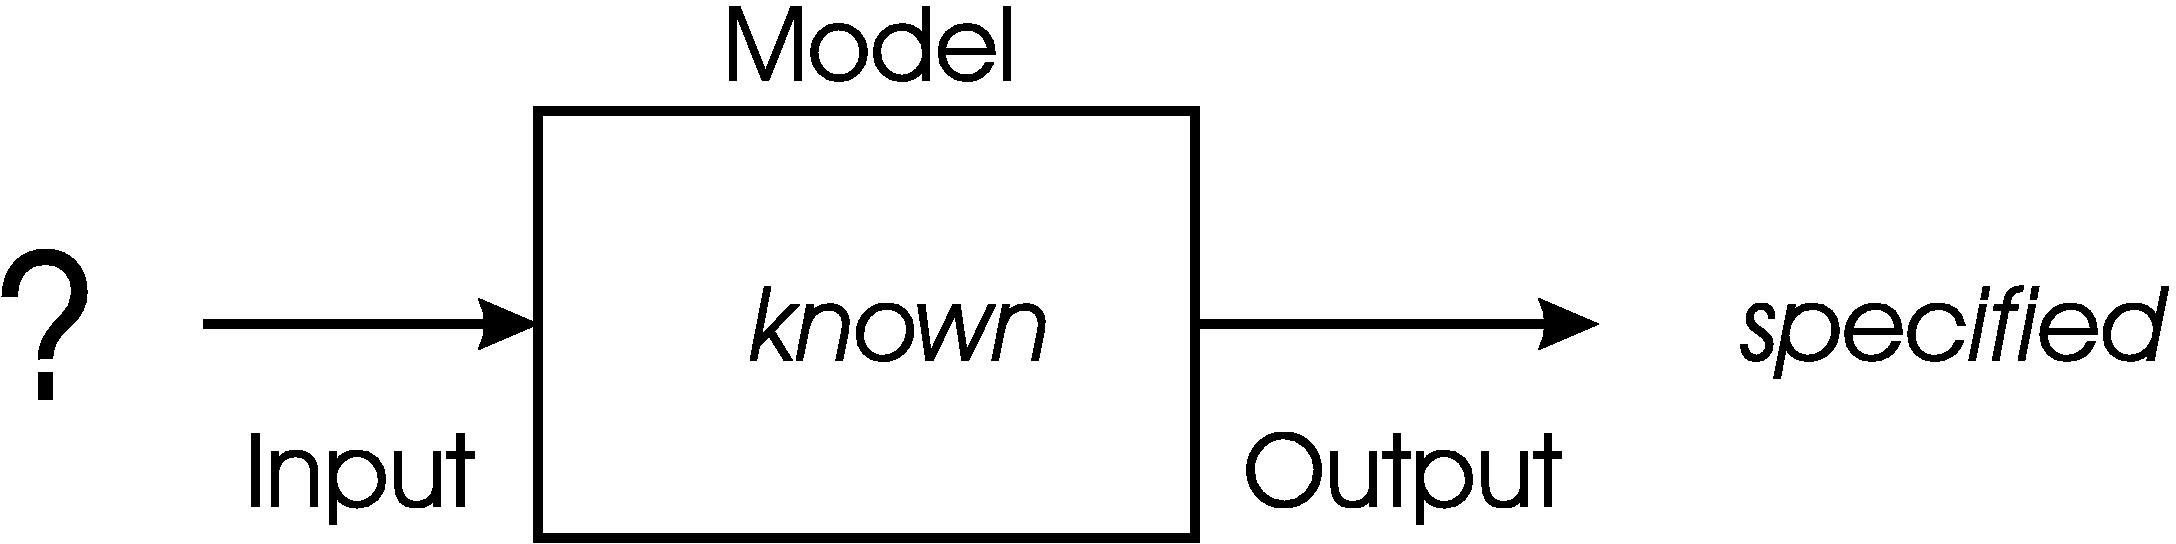
\includegraphics[width=4in]{intro/1-4.jpg}
\caption{\label{fig:ch1-4}Optimització d'entrada}
\end{figure}
\begin{figure} \centering 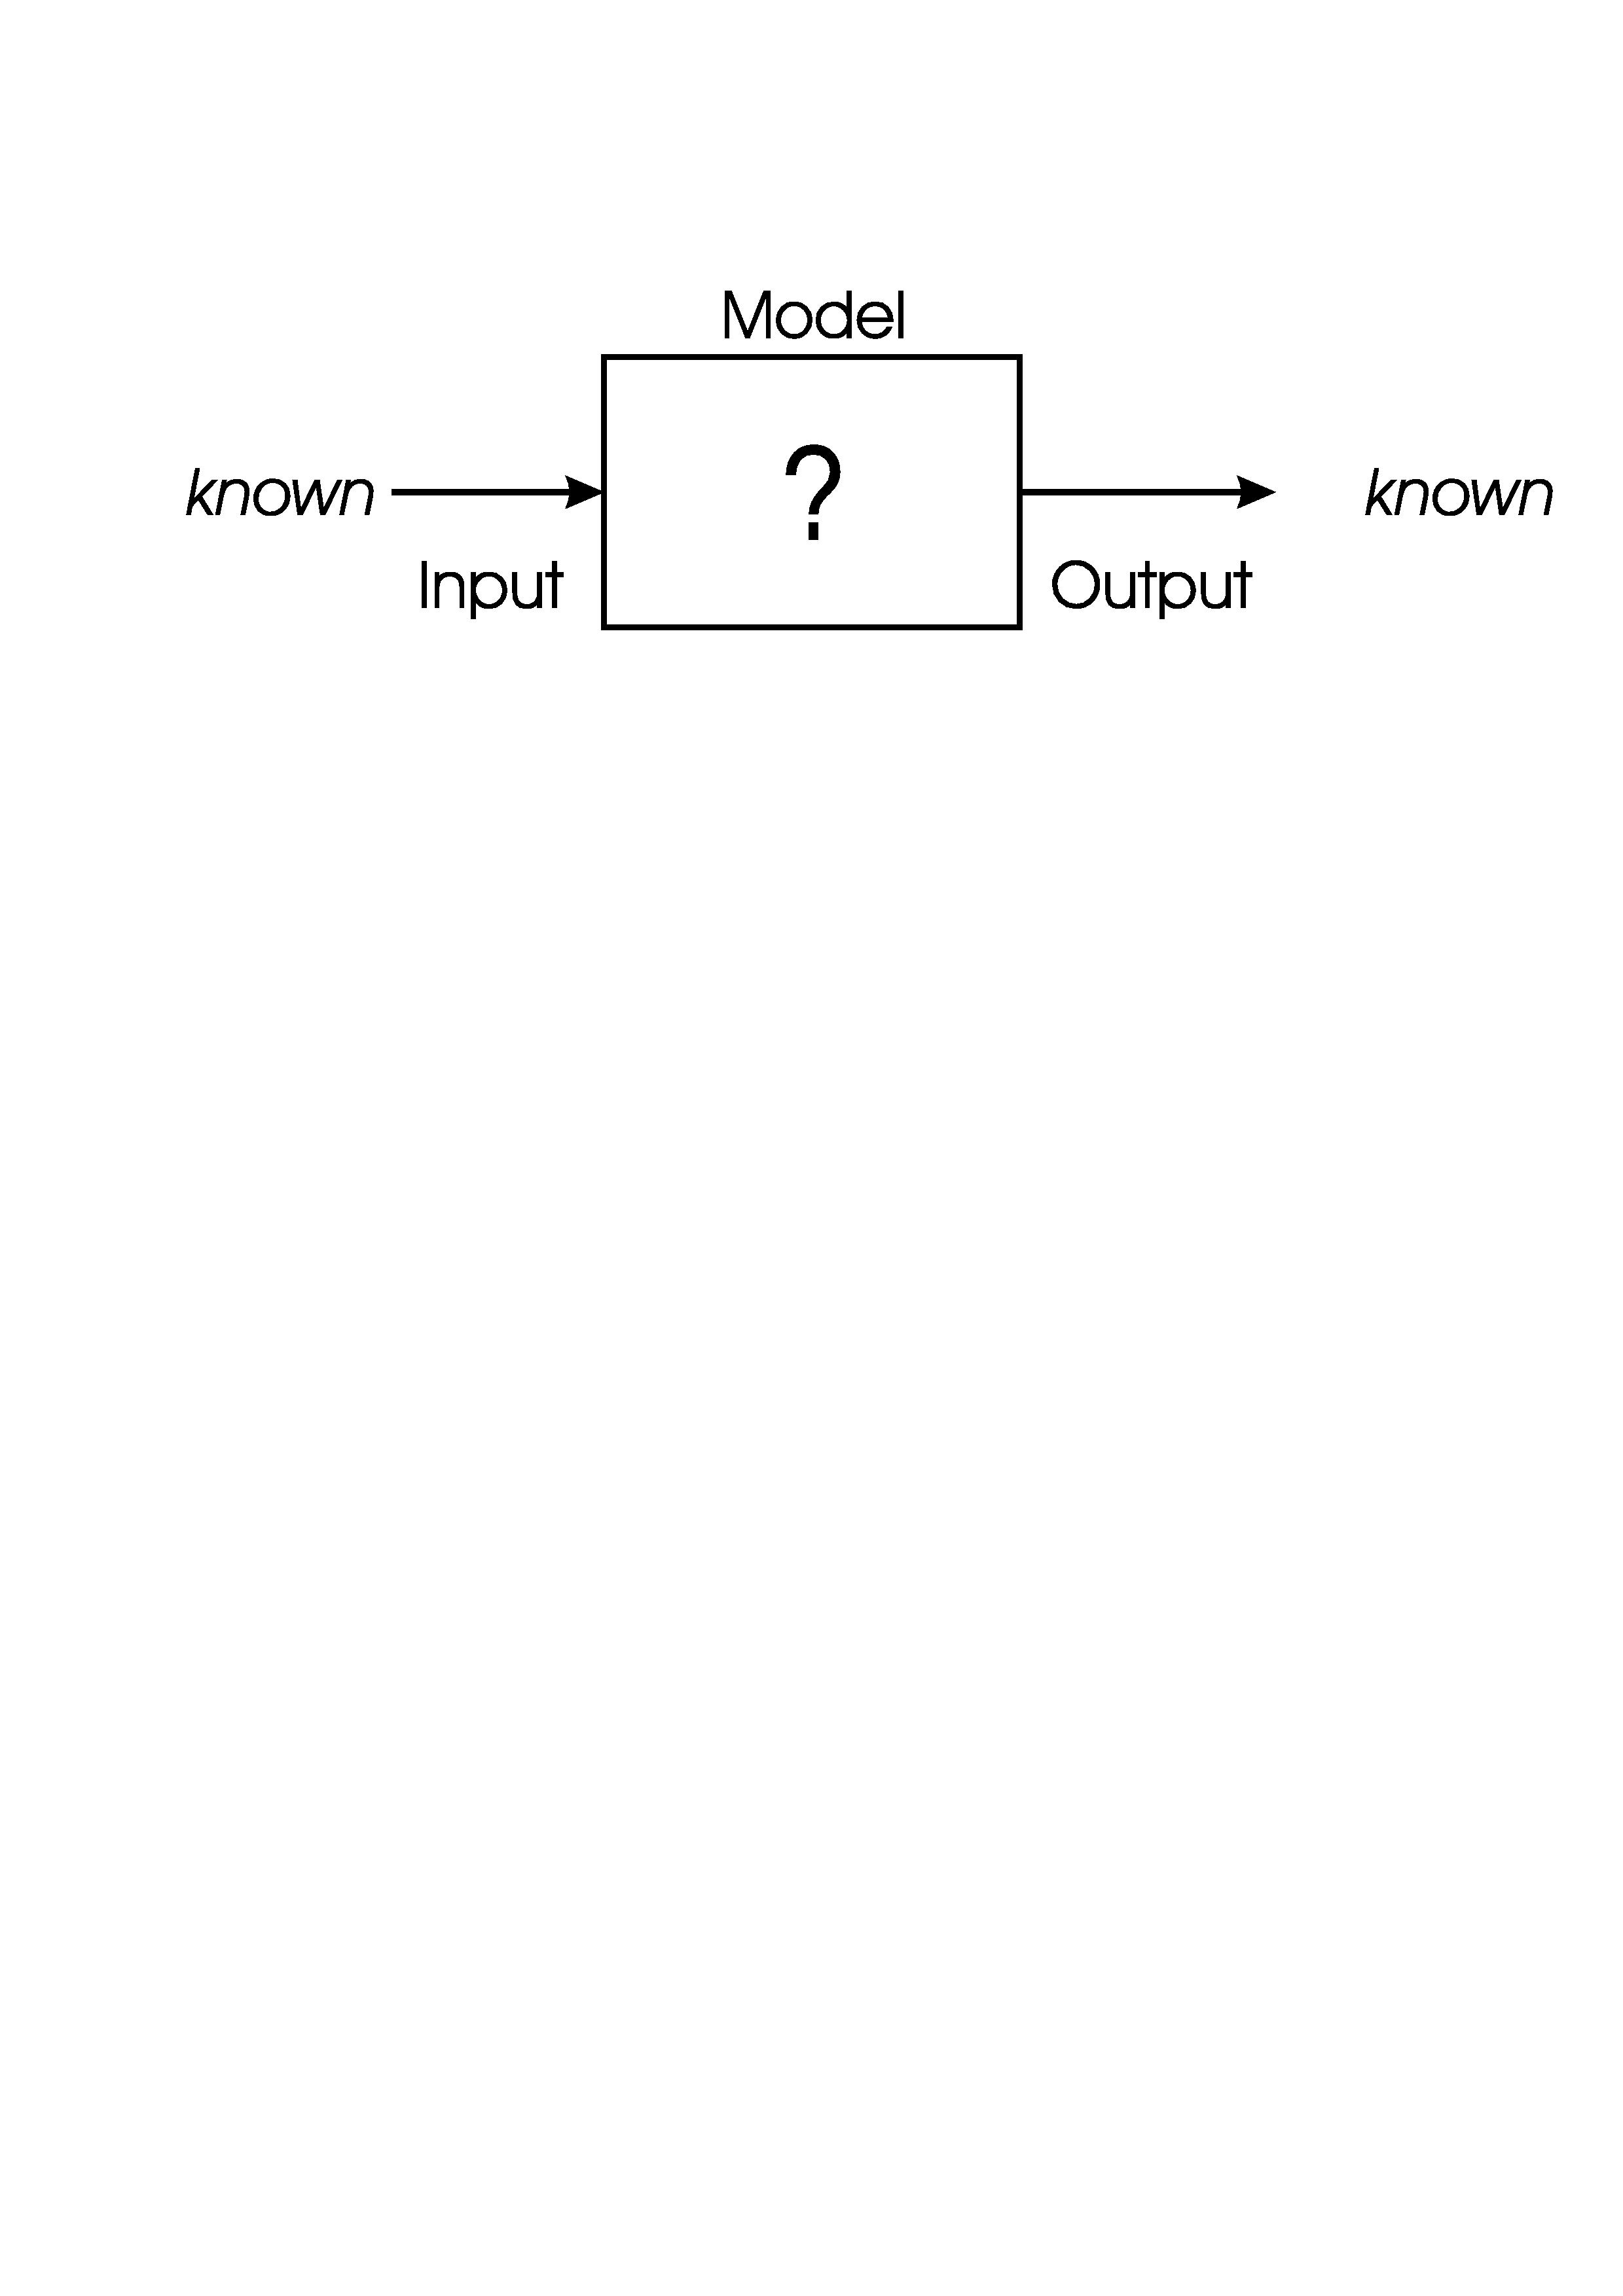
\includegraphics[width=4in]{intro/1-5.jpg}
\caption{\label{fig:ch1-5}Optimització procés}
\end{figure}

Els processos que s'intenten optimitzar, contenen, és clar, molta més informació
que en un dels algorismes genètics dels que s'han vist fins ara.  Això és
evident, ja que aquí, els individus són parts funcionals d'un sistema i no
només dades que un sistema agafarà i avaluarà.  Tot seguit es mostren tres
exemples de possibles problemes que es poden optimitzar:

\begin{itemize}
	\item Fórmules lògiques (per exemple $ (x\land true) \rightarrow ((x \lor y)
		\lor (z \leftrightarrow ( x \land y)))$ ). Figura \ref{fig:6-2-2}.
	\item Fórmules aritmètiques (per exemple $2\times\pi+((x+3)-\frac{y}{5+1})$
		).  Figura \ref{fig:6-2-1}
	\item Programes 
		\begin{verbatim}
				i = 1;
				while (i<20){
					i = i + 1;
					}
		\end{verbatim}. Figura \ref{fig:6-3}.
\end{itemize}

\begin{figure} \centering 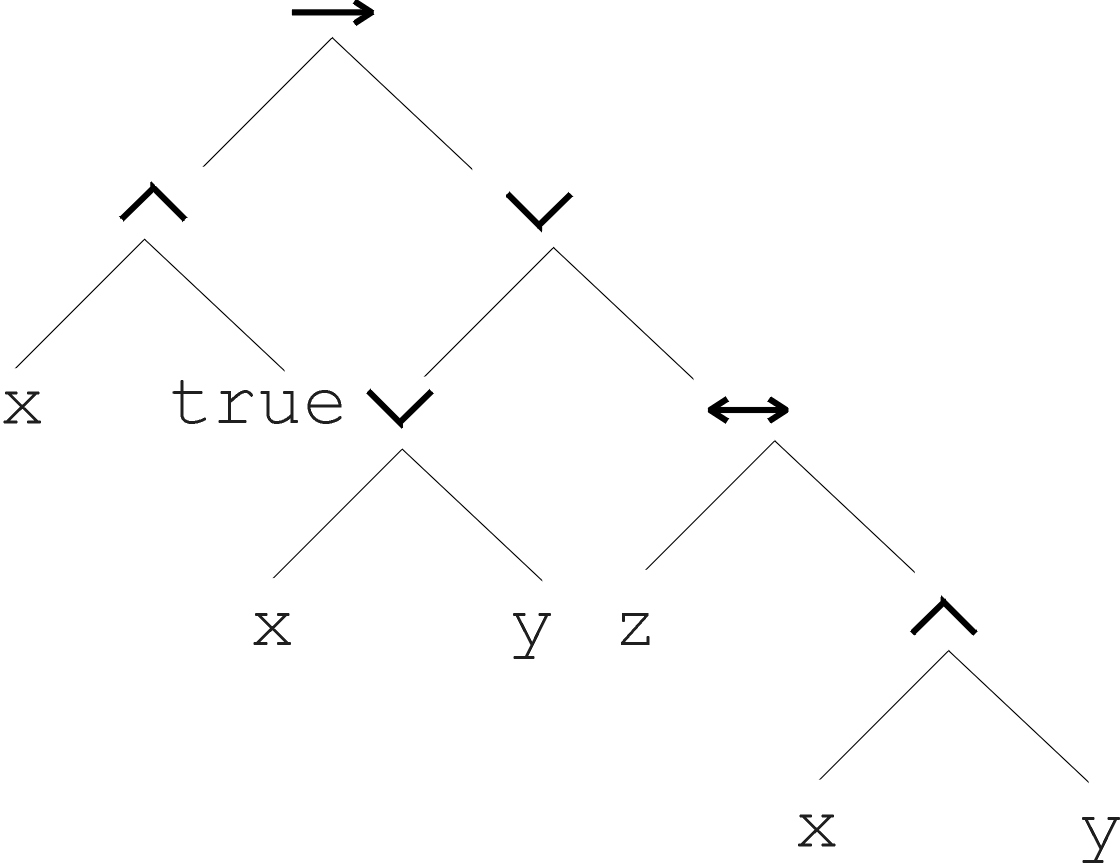
\includegraphics[width=4in]{intro/6-2-2.jpg}
\caption{\label{fig:6-2-2}Fórmula logica}
\end{figure}

\begin{figure} \centering 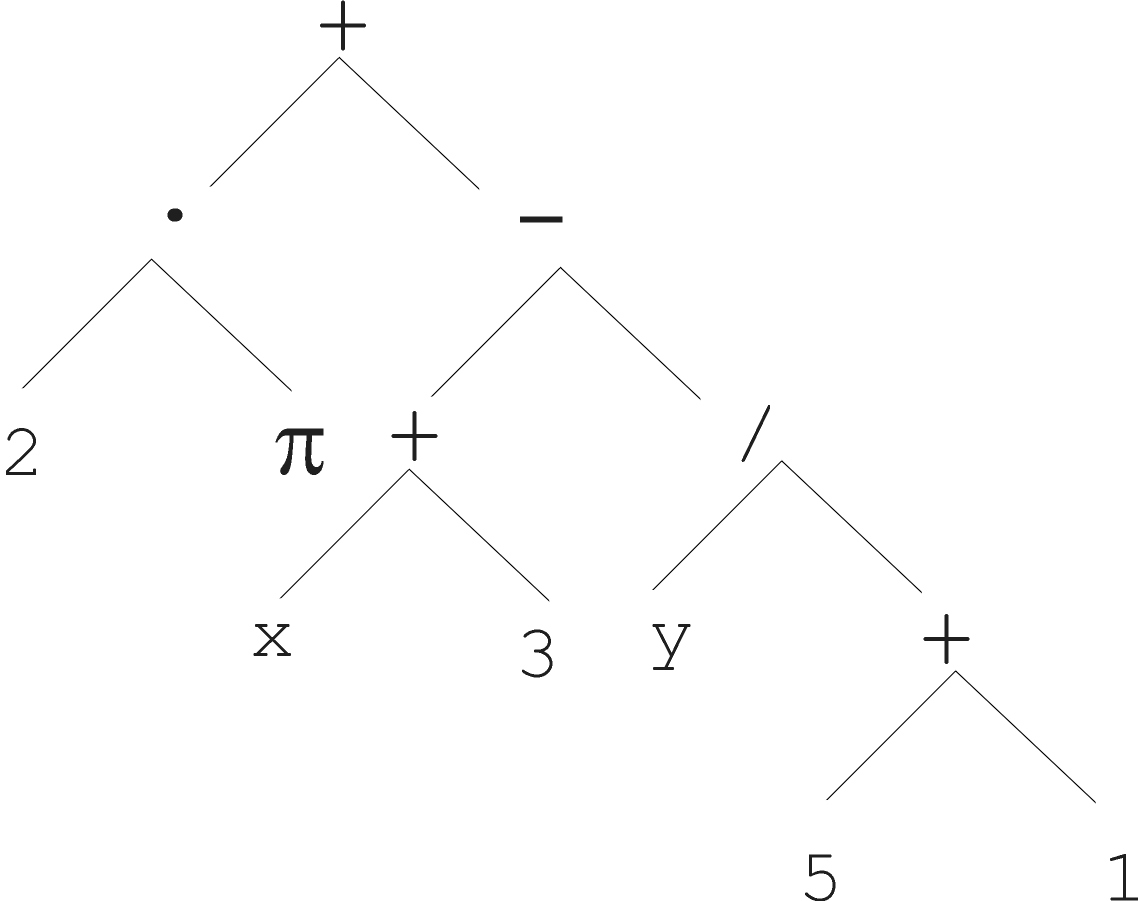
\includegraphics[width=4in]{intro/6-2-1.jpg}
\caption{\label{fig:6-2-1}Fórmula aritmètica}
\end{figure}

\begin{figure} \centering 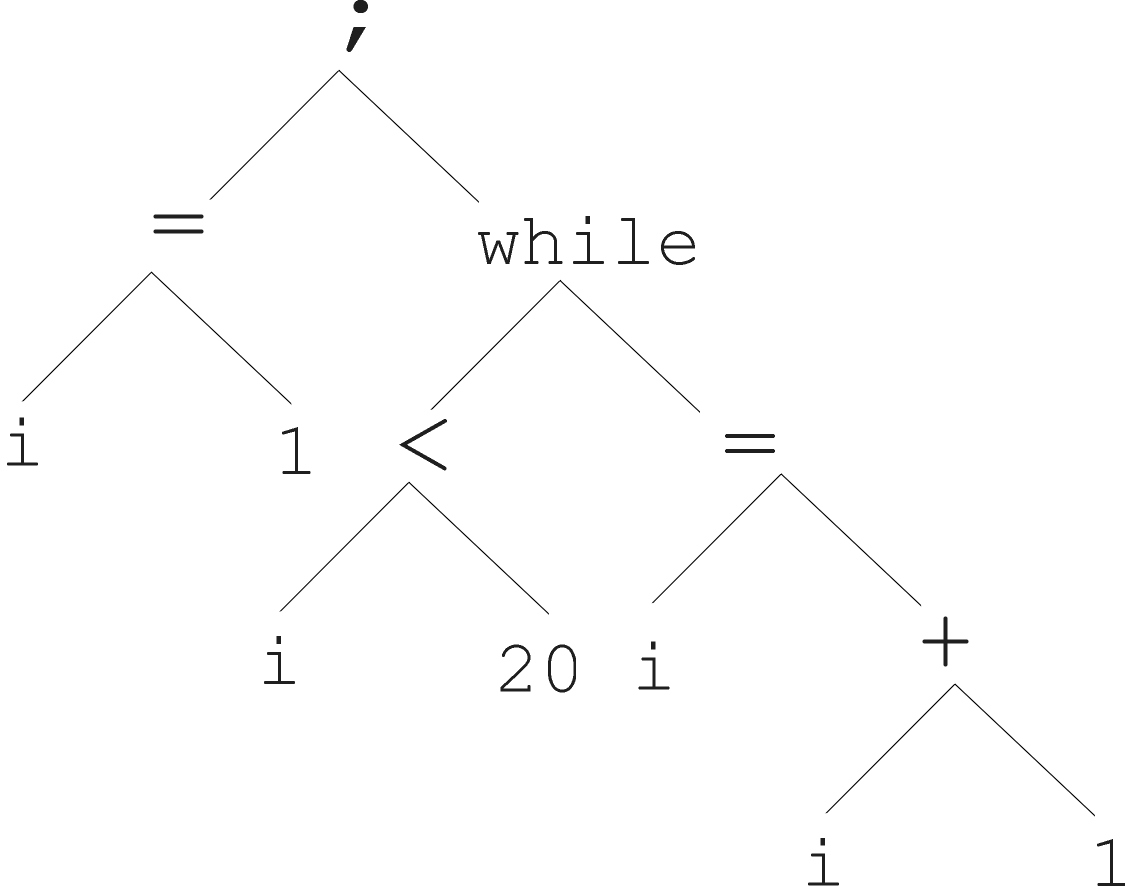
\includegraphics[width=4in]{intro/6-3.jpg}
\caption{\label{fig:6-3}programa}
\end{figure}

En aquest tipus d'algorismes, els individus no poden ser codificats com a un
sol vector de bits o reals, i aquests ser tractats independentment uns dels
altres, sinó que el que han de codificar els individus són arbres.  Per tant,
la seva codificació és més complexa, havent-hi una clara separació entre genotip
i fenotip.

Estrictament parlant, però, no hi ha cap altra diferència entre els GA clàssics
i GP o GEP.  Simplement, aquí interpretem els cromosomes com a arbres.

A continuació es farà una breu introducció a GP, per saber els orígens de
GEP, i seguirà una explicació una mica més detallada de GEP, que és la tècnica
que s'ha utilitzat en \texttt{GEP}.

\subsection{Antecessors: Programació Genètica} % (fold)
\label{sub:Ant. Programacio Genetica}
La programació genètica és una de les diferents disciplines dins dels algorismes
evolutius, inventat per Cramer en el 1985 (\cite{C85}) i després millorat per
Goldberg (\cite{Goldberg:89}) i
John Koza en 1992 (\cite{koza:92}) basat en la solució de problemes amb genotips de
llargada fixa, però interpretats de forma no lineal (arbres) de mida i formes.

Els individus en GP, normalment tenen un alfabet més ric que els algorismes
evolutius clàssics, però aquesta riquesa que ofereix tractar els cromosomes amb
una interpretació no lineal, fa que aquests individus no siguin autònoms, i no
poden funcionar com a genotip i fenotip alhora, ja que han de passar per una
fase de ``traducció''.

Per poder diferenciar la programació genètica de la programació d'expressions
genètiques, fem un repàs molt ràpid dels operadors més comuns en GP.

\subsubsection{Operadors} % (fold)
\label{ssub:operadors}

Els algorismes de programació genètica tenen els mateixos operadors que els
altres AE, però amb la diferència notable que s'ha de tenir en compte que al fer
una modificació sobre el genotip, el fenotip pot veure's modificat de manera
``no prevista'' si no anem molt en compte.  Per exemple, al fer un creuament
entre dos individus, el cromosoma resultant, pot no mantenir cap (o gairebé
cap) característica dels seus pares, donada la no-linealitat dels fenotips
respecte els genotips.  Això dona lloc a que molts dels individus generats a
partir de individus vàlids, són invàlids en el sentit que poden no complir les
condicions bàsiques per a ser traduïts a fenotips i posteriorment avaluats.

Una manera de assegurar que les propietats dels progenitors es mantenen a la
descendència i que continuen essent individus vàlids, és aplicar els operadors
a nivell de fenotip, i assegurant-se que els fills continuen tenint una mínima
entitat que els fa avaluables en el context del problema.  Això dificulta molt,
però, la programació dels operadors.

Per exemple, en el cas d'interpretar els genotips com a arbres amb formules
matemàtiques, al fer creuaments podem fer-los per subarbres, agafant l'arrel i
el fill esquerra del arbre d'un dels dos progenitors, i el fill dret de l'altre.
Tot seguit es comenten els dos operadors més interessants en programació
genètica.

\paragraph{Mutacions} % (fold)
\label{par:Mutacions}
Les mutacions en programació genètica són similars conceptualment a les que
trobem en els altres algorismes evolutius, canviant un subarbre aleatori del
cromosoma per un altre subarbre generat aleatòriament.  Veiem aquí la diferència
necessària en la implementació, ja que la mutació té lloc en l'espai del fenotip
(arbre) i no pas en el genotip (vector de símbols).  Hi ha hagut controvèrsia
sobre la aplicació de mutacions en programació genètica des de els seus inicis.
Koza en \cite{koza:92} aconsellava desactivar per complet la mutació.   Més
endavant, s'ha anat donant una mica més importància, però sense ser mai un
operador fonamental, donat que el creuament també actua en certa manera
d'operador de mutació però a més gran escala.  Aquestes mutacions canvien la
mida dels cromosomes.
% paragraph Mutacions (end)

\paragraph{Creuament} % (fold)
\label{par:Creuament}
El creuament de cromosomes en programació genètica és un operador binari que
consisteix en intercanviar dos subarbres entre dos cromosomes d'una població.
Una altra vegada, perquè el creuament no doni lloc a elements sintàcticament
incorrectes, el creuament s'ha de realitzar a nivell d'arbre, provocant també
canvis en la mida dels cromosomes.

% paragraph Creuament (end)

% subsubsection operadors (end)
% subsection Ant. Programació Genètica (end)

\subsection{Principis bàsics} % (fold)
\label{sub:Principis Basics}

La programació genètica, però, té alguns problemes fonamentals, que mermen la 
seva potència, com són el sobreentrenament (és molt fàcil obtenir 
solucions sobreentrenades per al conjunt de mostres amb el que entrenem
 l'algorisme), el \emph{bloat} (els arbres, tendeixen a créixer desmesuradament),
o bé la mateixa complexitat que té fer els creuaments o mutacions a nivell de 
fenotip. GEP, intenta solucionar alguns d'aquests problemes.


En GEP, els principals elements son els cromosomes i els arbres d'expressions,
on els segons són la expressió del la informació genètica codificada en els
cromosomes.  Com en la natura, el procés de descodificació s'anomena
\emph{traducció}.

La correspondència d'un a l'altre ha de ser unívoca i hi ha unes regles que ens
permeten passar d'un a l'altra.  En la natura, aquesta traducció no és pas tant
fàcil, ja que no se sap gairebé res del genotip, si tenim només un fenotip, però
per a tenir una traducció fàcil dins de GEP, es disposa d'una notació anomenada
\emph{Karva Notation} que ens permet fer les traduccions en les dues direccions
fàcilment \ref{ssub:Notacio Karva}.

% explicar constants


%http://www.gene-expression-programming.com/Tutorial002.asp
\subsubsection{Notació Karva} % (fold)
\label{ssub:Notacio Karva}

La notació Karva, és una manera de representar qualsevol expressió matemàtica o
lògica en una estructura lineal de manera que es pugui traslladar a un arbre
fàcilment \cite{ferreira:2001} i \cite{ferreira:2006}.

Les estructures lineals que conformen els individus en GEP són els cromosomes,
i cada cromosoma té un o més gens, que aquí prenen un altre significat més
ampli, no referint-se als ``àtoms'' indivisibles (com en els AE que hem vist
fins ara) sinó que cada gen està associat a una K-expression.
\cite{ferreira:2007}

Tot seguit es mostra un exemple d'un gen, i en \ref{fig:expression tree1} el seu
\texttt{Arbre d'expressió} equivalent

\begin{center}
0123456    
+/*abcd
\end{center}

\begin{figure}[h]
\begin{center}
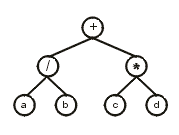
\includegraphics{intro/et1.png}
\end{center}
\caption{Arbre d'expressió}
\label{fig:expression tree1}
\end{figure}

La traducció d'un a l'altre és directe.  El primer element en el gen (posició
0) correspon a la arrel del arbre.  Llavors, sota d'aquest node, s'enganxen
tants nodes fills com arguments tingui la funció representada pel node arrel
(dos en aquest cas). Els nodes fills es van omplint recursivament, consumint
símbols del cromosoma, fins que un nivell del arbre queda només omplert per
nodes terminals, que no son més que nodes on el símbol que contenen té aritat
zero.

Més formalment, tant el gen com l'arbre \ref{fig:expression tree1} poden ser
representats per la expressió matemàtica:

	$\frac{a}{b}+c \times d$

Per assegurar que els arbres que es creïn siguin sintàcticament vàlids, es
divideix un gen en dues parts, amb mides que segueixen unes normes determinades
que s'expliquen en detall en l'apartat \ref{ssub:Inicialitzacio}.  Un gen es
composa de la primera part (\emph{head}) que conté funcions i terminals, i d'una
segona part (\emph{tail}) que només conté terminals (aritat zero). Si el tail és
suficientment llarg com per omplir la última capa del arbre que genera el propi
gen, sempre hi haurà prou operands per a donar a les funcions.

% subsubsection Notació Karva (end)

\subsubsection{Individus} % (fold)
\label{issub:individus}
% subsubsection individus (end)

Com s'ha explicat en \ref{ssub:Notacio Karva}, els individus son representats en
una tira de símbols (genotip), però al interpretar-los i avaluar-los, tenen una
representació en forma d'arbre d'expressió similar a un AST\footnote{Abstract
syntax tree}.

Un individu o cromosoma està format per un o més gens.  En la versió més
primària, un cromosoma conté només un gen, però es poden combinar diversos gens,
creant cromosomes multigen, com s'explicarà més endavant.

En aquest tipus de notació, existeixen el que denominem ``zones
no-codificadores'', que són parts del gen, que per diversos motius formen part
del genotip, però no tenen representació, ni es mostren en el fenotip.  Un
exemple d'això és


\begin{verbatim}
	01234567890123456 	 
	Q/a*+b-cbabaccbac
\end{verbatim}

On la $Q$ representa l'arrel quadrada.  En aquest gen, té el i \emph{head} (que ocupa
de la posició 0 a la 7) de llargada, i el tail (de la 8 a la 16) de llargada 9.
El head té tan funcions com terminals, i el tail, només té terminals.

La codificació d'aquest gen es mostra en \ref{fig:unfinished} mostra com en aquest cas,
no han fet falta tots els elements del gen per a construir l'arbre.  Això és
perquè la fórmula que en assegura tenir prou tail, preveu el pitjor dels casos,
essent tots els elements del head funcions amb la màxima aritat.  Com que en
aquest cas, tenim una arrel quadrada (i en l'arrel del arbre), deixem de
necessitar gairebé la meitat del gen per a fer la traducció.

\begin{figure}[h]
\begin{center}
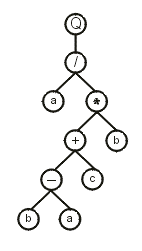
\includegraphics{geptut/pt02.png}
\end{center}
\caption{Arbre d'expressió}
\label{fig:unfinished}
\end{figure}

Aquests trossos de cromosoma que no s'utilitzen, participen igualment en els
creuaments (es fan a nivell de vector de símbols), i fan que una mutació en una
zona del \emph{head} ``activi'' una zona prèviament inactiva.  Això dona tant
als creuaments com a les mutacions molta més versatilitat que en els algorismes
clàssics.

Aquesta elegància de la programació d'expressions genètiques és la clau del
funcionament de GEP.  La codificació Karva és el nucli del bon funcionament de
GEP, però és només el principi.  És a dir, existeixen mètodes més avançats que
parteixen d'aquesta base, i aconsegueixen millorar els resultats del GEP
estàndard, com per exemple, codificar més d'un gen en un cromosoma. Són els
anomenats cromosomes multigen.  En aquests sistemes, els cromosomes estan
codificats a partir de diversos gens, i cadascun d'ells formen un subarbre o
subprograma.  Una vegada traduïts cadascun dels subarbres, aquests poden ser
connectats entre ells de diferents maneres.  Una de les més utilitzades és usant
funcions especials, anomenades d'enllaç. Aquestes funcions uneixen linealment
els diferents subarbres per ordre d'aparició en el gen.  Per exemple, observem
el següent cromosoma, composat per tres sub-gens.
	%XXX

	\begin{center}
	\begin{verbatim}
	012345678012345678012345678 	 
	*aQ+abbaa/Q*/aababa*+Qaabba
	\end{verbatim}
	\end{center}


Aquest cromosoma codifica tres arbres de la Figura \ref{fig:tres sub-et}

\begin{figure}[h!]
\begin{center}
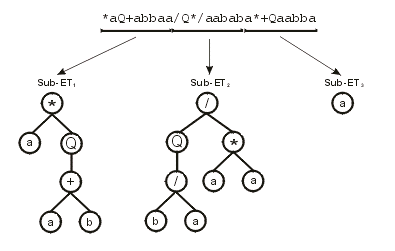
\includegraphics{geptut/pt03a.png}
\end{center}
\caption{Cromosoma representant tres sub-arbres}
\label{fig:tres sub-et}
\end{figure}

Si s'utilitzen funcions d'enllaç, per exemple, la suma, la avaluació del
cromosoma complet passaria a ser el mostrat en la figura 
\ref{fig:tres sub-et amb link}

\begin{figure}[h!]
\begin{center}
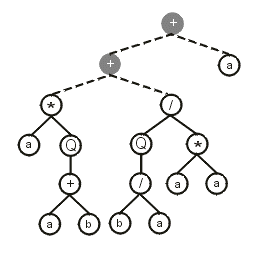
\includegraphics{geptut/pt03b.png}
\end{center}
\caption{Representació dels tres sub-arbres enllaçats amb la operació suma}
\label{fig:tres sub-et amb link}
\end{figure}

La implementació del individu que hem programat ha estat una versió una mica més
avançada que la de les funcions d'enllaç, que utilitza un dels subarbres, com a
metadada, on els terminals no es refereixen a terminals de la funció, sinó que
són referències als altres subarbres, que sí tenen com a fulles les entrades de
la funció objectiu.

%XXX
%\subsubsection{Esquema Bàsic} % (fold)
%\label{ssub:Esquema Basic}
%% subsubsection Esquema Bàsic (end)

%\subsubsection{Funció d'avaluació} % (fold)
%\label{ssub:funcio d'avaluacio}
%% subsubsection funció d'evaluació (end)
%% subsection Principis Bàsics (end)

\subsection{Operadors} % (fold)
\label{sub:Operadors}

Tot seguit es descriuran els operadors usats en GEP, sense concretar la seva
implementació, sinó explicant com varien els individus.  Per a veure els
detalls sobre la aplicació en aquest projecte, les explicacions i
implementacions més complertes consultar la secció \ref{cha:GEP}.

\subsubsection{Inicialització} % (fold)
\label{ssub:Inicialitzacio}
Donades les particularitats de la notació Karva, la inicialització d'arbres
aleatoris, consisteix en omplir head i tail amb símbols aleatoris permesos en
cadascuna de les zones.  Normalment, el head tindrà símbols operadors i
variables terminals i el tail, únicament contindrà variables terminals.  La
aritat zero dels terminals ens garantitza que l'arbre serà sintàcticament
correcte.

La població inicial es genera aplicant aquest algorisme a cadascun dels
individus.
% subsubsection Inicialització (end)

\subsubsection{Selecció} % (fold)
\label{ssub:Seleccio}
En GEP, també s'utilitza, per norma general la selecció per ruleta
(secció \ref{subs:Iseleccio}).  Un individu té una probabilitat de ser seleccionat per a
la reproducció proporcional al seu fitness en valor absolut, respecte als altres
individus de la població.

% subsubsection Selecció (end)

\subsubsection{Creuament} % (fold)
\label{ssub:Creuament}

El creuament, juntament amb la mutació és l'element que dóna la major part de la
riquesa als algorismes GEP.  Els creuaments en GEP són uns operadors que, a
diferència de la programació genètica, donen molta llibertat per a la
experimentació, ja que només s'han de mantenir unes certes regles molt bàsiques,
i es pot assegurar que es generaran arbres sintàcticament correctes.

Per exemple, en GEP es poden aplicar creuaments típics dels algorismes evolutius
clàssics, com el \texttt{creuament per un punt}, o els \texttt{creuaments per
diversos punts}, ja que si no variem la mida de la descendència, sempre es
mantindran certes les regles de què el tail no contingui mai operands (nodes
d'aritat $>0$).

A més a més, GEP té uns creuaments particulars, anomenats \texttt{recombinació
de gens}, que es basen en separar els dos individus a creuar en els seus
diferents gens, i fer el creuament ajustant els punts de tall als límits dels
gens.  Aquest creuament només és aplicable si implementem individus multigen.
% subsubsection Creuament (end)

\subsubsection{Mutació} % (fold)
\label{ssub:Mutacio}
Les mutacions, igual que els creuaments, també es poden dividir en dos
subconjunts, els que són totalment portables del món dels AE clàssics, i els
particulars de GEP.

Una mutació dels AE clàssics pot ser, per exemple, l'alteració d'un símbol
aleatori.  L'únic que s'ha de tenir en compte, és quina posició del gen s'està
mutant, per a no incloure en el tail símbols que estan restringits a usar-los
només en el head.

Per altra banda, GEP disposa de tres mutacions pròpies, anomenades IS, RIS i
``translació de gen'', que es basen en desplaçaments de conjunts de símbols al
llarg del gen.  Aquests operadors estan explicats més en detall a \ref{par:IS},
\ref{par:RIS} i \ref{par:Translacio de gen}
% subsubsection Mutació (end)

\subsubsection{Reemplaçament} % (fold)
\label{ssub:Reemplacament}

Pel reemplaçament tmabé s'utilitza elitisme, on mantenim el millor dels
individus per a la següent generació.  Les poblacions no cambien de 
mida.

% subsubsection Reemplaçament (end)
% subsection Operadors (end)
% section Programació d'expressions genètiques (end)

\section{Estat de l'art} % (fold)
\label{sec:Estat de l'art}

Actualment, els algorismes genètics estan essent més i més utilitzats no sols en
el món acadèmic, sinó també en el món de l'empresa. 


Les últimes publicacions referents a algorismes genètics tendeixen cap a
optimitzacions de la convergència.  Els algorismes genètics són processos
estocàstics (la durada o nombre d'iteracions fins a aturar-se no és un valor
conegut a priori).  Així doncs, el que s'intenta és aconseguir ``guiar''
l'algorisme perquè avanci de pressa cap a un estat convergent (s'aturi), sense
perjudicar això a la eficàcia.  Molts dels estudis de tècniques per millorar
l'eficiència dels algorismes genètics estan relacionats amb l'aprofitament de la
paralelització de processos, aprofitant sistemes distribuïts, o fins i tot en
cloud.  

Els treballs més recents relacionats amb algoritmes evolutius estan relacionats
amb la utilització de entorns de treball (frameworks) i paradigmes de
programació paralela, com poden ser hadoop o MapReduce \cite{VLCG09}.

\subsection{Tecnologia} % (fold)
\label{sub:Tecnologia}

Des dels inicis de la programació, el llenguatge per excelència
relacionat amb la intel·ligència artificial ha estat lisp \cite{JMC59}, creat per John
McCarthy el 1958 donat la gran flexibilitat que oferia (a més, en aquells temps
hi havia fortran com a alternativa, un llenguatge molt més rígid).  Així doncs,
els majors avenços relacionats amb la IA han tingut gairebé sempre les seves
primeres implementacions en Lisp o derivats (Scheme).  

El ``problema'' dels llenguatges tant dinàmics com Lisp, era que al treballar sobre
màquina virtual eren massa lents per a la implementació en producció.  Recordem que les
aplicacions que utilitzen algorismes de intel·ligència artificial requereixen un
gran volum de càlculs.

És per això que els sistemes amb grans necessitats de càlcul per a producció
normalment s'implementen amb llenguatges ``propers al ferro'' com poden ser
C/C++. 

Actualment i donada la gran potència de calcul dels ordenadors actuals, cada
vegada hi ha més empreses que comencen a utilitzar llenguatges interpretats per
a realitzar algorismes genètics. Llenguatges com Haskell i Erlang que han
demostrat ser molt ràpids i paralelitzables, no han fet el salt a la
intel·ligència artificial massivament, ja que la seva puresa (transparència
referencial i fortament tipats) els fa més ferragosos de treballar en problemes
eminentment dinàmics com els algoritmes evolutius.

% subsection Tecnologia (end)
% section Estat de l'art (end)

%\bibliographystyle{unsrt} 
%\bibliography{bibliografia}


%\end{document}

